%----------------------------------------------------------------------------------------
%	SECTION 1
%----------------------------------------------------------------------------------------

\section{Geometric Representations of Matroids of Small Rank.}

\begin{definition}
    Let $V$ be a vector space over a field $F$ of dimension $m$, a set of
    vector $\{v_1, \dots, n_k\}$, not all necessarily distinct, is called
    \textbf{affinely dependent} if there exists scalars $a_1, \dots, a_k \in F$,
    not all $0$ such that
    \begin{equation*}
        a_1v_1+\dots+a_kv_k=0
    \end{equation*}
    and
    \begin{equation*}
        a_1+\dots+a_k=0
    \end{equation*}
    We call $\{v_1, \dots, v_k\}$ \textbf{affinely independent} if they are not
    affinely dependent.
\end{definition}

We present one lemma on affine independence without proof.

\begin{lemma}\label{1.5.1}
    A set $\{v_1, \dots. v_k\}$ of vectors (not necesarily distinct) of a
    vector space $V$ of dimension $m$ is affinely dependent if the set of
    vectors $\{(1,v_1), \dots, (1,v_k))\}$ is linearly dependent in the vector
    space $F^{m+1}$.
\end{lemma}
\begin{corollary}
    $\{v_1, \dots, v_k\}$ is affinely independent if $\{(1,v_1), \dots,
    (1,v_k))\}$ is linearly independent.
\end{corollary}

\begin{lemma}\label{1.5.2}
    Let $V$ be a vector space of dimension $m$ over a field $F$, and let  $E$
    be the set of vectors of $V$, not all necesarily distinct. If $\Ic$ is the
    collection of all subsetets of  $E$ which are affinely independent, then
    $E$ together with  $\Ic$ forms a matroid.
\end{lemma}
\begin{proof}
    By lemma \ref{1.5.1}, we have that $M=M[A]$ where $A$ is the  $(m+1) \times
    n$ matrix over $F$ whose columns are  $(1,v_i)^T$.

    Alternatively, if we prove this directly by definition, we see that
    $\emptyset \in \Ic$, since  $\emptyset$ is affinely independent. Moreover,
    if  $\{v_1, \dots, v_k\}$, is affinely independent, then
    $a_1v_1+\dots+a_kv_k$ with $a_1+\dots+a_k=0$ implies that $a_i=0$ for each
    $1 \leq i \leq k$, then indexing  $1 \leq j \leq i$, we get that the subset
    $\{u_1, \dots, u_j\}$ of $\{v_1, \dots, v_k\}$ is also affinely independnet.

    Now suppose that $U=\{u_1, \dots, u_k\}$, and $V=\{v_1, \dots, v_n\}$ are
    affinely independnet, with $k>n$, so that  $|U|<|V|$. Then by definition, we
    have that
    \begin{align*}
        a_1v_1+\dots+a_kv_k=0,  &&   a_1+\dots+a_k=0 \\
    \end{align*}
    implies $a_i=0$ for ech $1 \leq i \leq k$, and
    \begin{align*}
        b_1u_1+\dots+b_nu_n=0,  &&  b_1+\dots+b_n=0
    \end{align*}
    implies $b_j=0$ for ech $1 \leq j \leq n$

    Then choose a vector $v_i \in \com{V}{U}$, so that $v_i \neq u_j$ for all
    $u_j$ of  $U$. Then we find that:
    \begin{align*}
        (b_1u_1+\dots+b_nu_n)+a_iv_i=0,  &&  (b_1+\dots+b_n)+a_i=0
    \end{align*}
    Since $v_i \in V$,  $a_i=0$, so that the set  $U \cup v_i$ is also affinely
    independent. Therefore $E$ forms a matroid having  $\Ic$ as its collection
    of independent sets.
\end{proof}

\begin{example}\label{1.17}
    \begin{enumerate}
        \item[(1)] Let $E=\{(0,0), (1,0), (2,0), (0,1), (0,2), (1,1)\}$ Of $\R^2$,
            and consider the affine matroid on $E$ We find that this matroid can
            be represented by the geometric figure in figure \ref{fig_1.9} below.
            \begin{figure}[h]
                \centering
                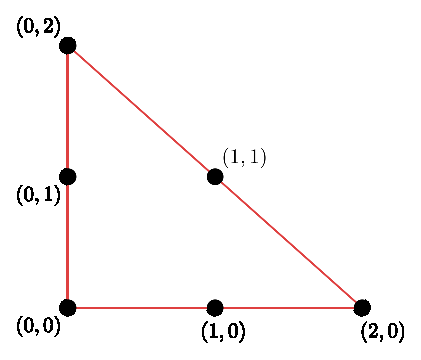
\includegraphics[scale=0.8]{Figures/chapter1/rank_3_affine_matroid.eps}
                \caption{An affine matroid of rank $3$.}
                \label{fig_1.9}
            \end{figure}

        \item[(2)] Consider the affine matroid on $\R^3$ with ground set
            $E=\{(0,0,0), (1,0,0), (1,1,0), (0,1,0), (0,1,1), \\ (0,0,1)\}$. We
            can geometrically represent this matroid by a wedge in $\R^3$ as in
            figure \ref{fig_1.10}
             \begin{figure}[h]
                \centering
                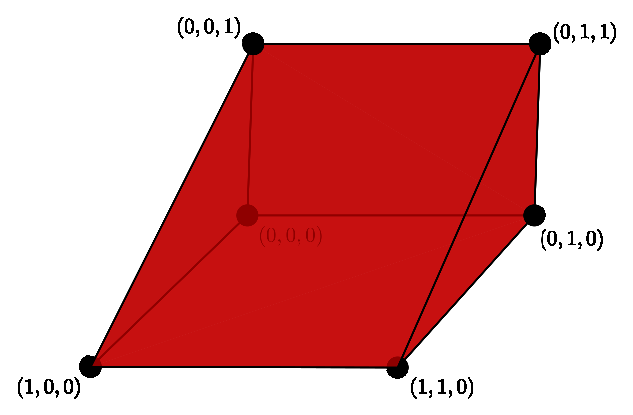
\includegraphics[scale=0.8]{Figures/chapter1/rank_4_affine.eps}
                \caption{A rank $4$ affine matroid in  $\R^3$.}
                \label{fig_1.10}
            \end{figure}
            The only dependent sets of less than $5$ points are the three
            $4$-point planes of the wedge.

        \item[(3)] Consider the $2 \times 5$ matrix:
            \begin{equation*}
                A=\begin{pmatrix}
                    1   &   0   &   0   &   1   &   1   \\
                    0   &   1   &   0   &   0   &   1   \\
                  \end{pmatrix}
            \end{equation*}
            Which defines a matroid $M[A]$ Labeling the columns of $A$ as
            $E=\{1,2,3,4,5\}$, we can represent this matroid geometrically in the
            following figure \ref{fig_1.11}. Here we represent the loops of $M[A]$ as
            graphical loops (elements adjecent to themselves in a graph), and we
            represent parallel elements by two tangent points.
            \begin{figure}[h]
                \centering
                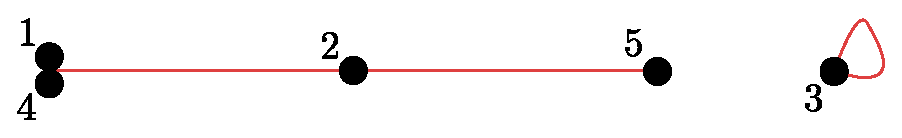
\includegraphics[scale=0.8]{Figures/chapter1/rank_2_matroid.eps}
                \caption{The rank $2$ matroid $M[A]$ on the matrix $A$.}
                \label{fig_1.11}
            \end{figure}
    \end{enumerate}
\end{example}

\begin{definition}
    Let $E$ be a set and $\Lc$ the collection of lines inducing a geomtry on
    $E$. We call a subset $X$ of $\Lc$ \textbf{geometrically} dependent if for
    any of the points of $X$, two are identical, three are colinear, four are
    coplanar, or there are  $5$ arbitrary points in space.
\end{definition}

\begin{theorem}\label{1.5.3}
    Affine dependence is equivalent to geometric dependence.
\end{theorem}

Theorem \ref{1.5.3} provides a way to represent matroids of small rank
geometrically. However, not all geometric figures are matroids. Consider the
next example.

\begin{example}\label{1.18}
    \begin{figure}[h]
        \centering
        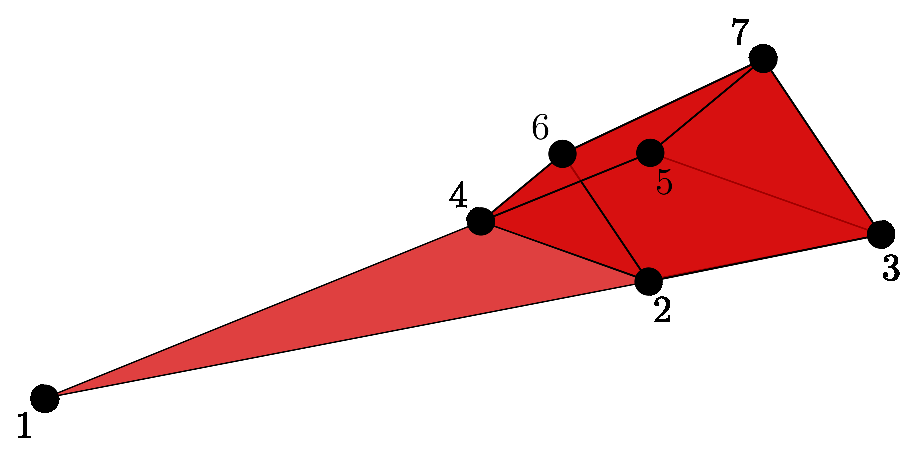
\includegraphics[scale=0.8]{Figures/chapter1/escher_matroid_1.eps}
        \caption{The Escher Figure.}
        \label{fig_1.12}
    \end{figure}
    Consider the geometric figure in figure \ref{1.12}. On notion of dependnece
    in geometry is that a set of points are dependent if they are colinear. Thus
    the sets $\{1,2,3\}$ and $\{1,4,5\}$ are dependent lines. The dependent
    planes are $\{2,3,4,5\}$, $\{2,3,6,7\}$, and $\{4,5,6,7\}$. However, this
    diagram does not represent a matroid. For, suppose to the contrary. Let
    $X=\{1,2,3,6,7\}$, and $Y=\{1,4,5,6,7\}$, then we have
    $\rank{X}=\rank{Y}=3$, and $\rank{(X \cup Y)}=4$, so we must have $\rank{(X
    \cup Y)}+\rank{(X \cap Y)} \leq \rank{X}+\rank{Y}$, so that $\rank{(X \cap
    Y)}=\rank{\{1,6,7\}} \leq 2$. However, $\{1,6,7\}$ are noncolinear, and
    hence independent, so that $\rank{(X \cap Y)}=3$, a contradiction. So to
    make figure \ref{fig_1.12} into a matroid, we would like to draw a line
    inbetween $1$ and  $7$ so that $1-6-7$ are colinear, as shown in figure
    \ref{fig_1.13}.
    \begin{figure}[h]
        \centering
        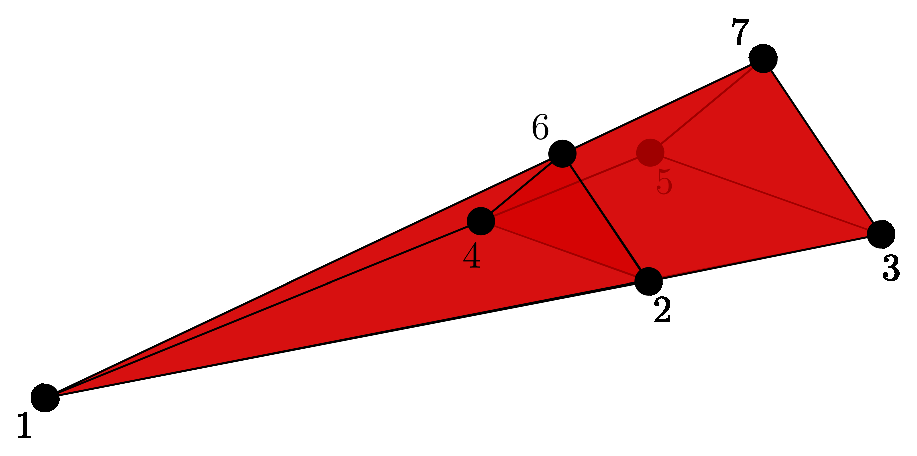
\includegraphics[scale=0.8]{Figures/chapter1/escher_matroid_2.eps}
        \caption{The Escher matroid.}
        \label{fig_1.13}
    \end{figure}

    We call the matroid in figure \ref{fig_1.13} the \textbf{Escher matroid}.
    Notice that the rank of this matroid is $4$.
\end{example}

The next result gives a way of identifing when geometric figures represent
matroids of rank at most $4$, provided that any two distinct lines in the
figure meet in at most one point.

\begin{lemma}\label{1.5.4}
    Let $E$ be a set and $\Lc$ a collection of subsets of $E$ each having
    atleast $3$ elements, and such that every two distinct members of $\Lc$
    intersect at atmost one element. Let  $\Ic$ be the collection of subsets $X$
    of  $E$ having atleast  $3$ elements, such that no member of  $\Lc$ contains
    on elements of  $X$. Then $E$ together with $\Ic$ forms a simple matroid $M$
    of rank  $\rank{M} \leq 3$, whose rank $1$ flats are the one element subsets
    of  $E$, and whose rank $2$ flats are the members of $\Lc$ together with all
    two element subsets $Y$ of $E$ such that no member of $\Lc$ contains $Y$.
\end{lemma}
\begin{corollary}
    Every simple matroid of $\rank \leq 3$ arises this way.
\end{corollary}

\begin{example}\label{1.19}
    Condsider the $7$ and  $13$ point figures of the projective geometries
    $PG(2,2)$ and $PG(2,3)$. By lemma \ref{1.5.3}, we get that $PG(2,2)$ and
    $PG(2,3)$ form $\rank=3$  matroids. Specifically, we call $PG(2,2)$, which is
    the smallest such projkective geometry, the \textbf{Fano plane}, and hence
    call the matroid on $PG(2,2)$ the \textbf{Fano matroid}.
    \begin{figure}[h]
        \centering
        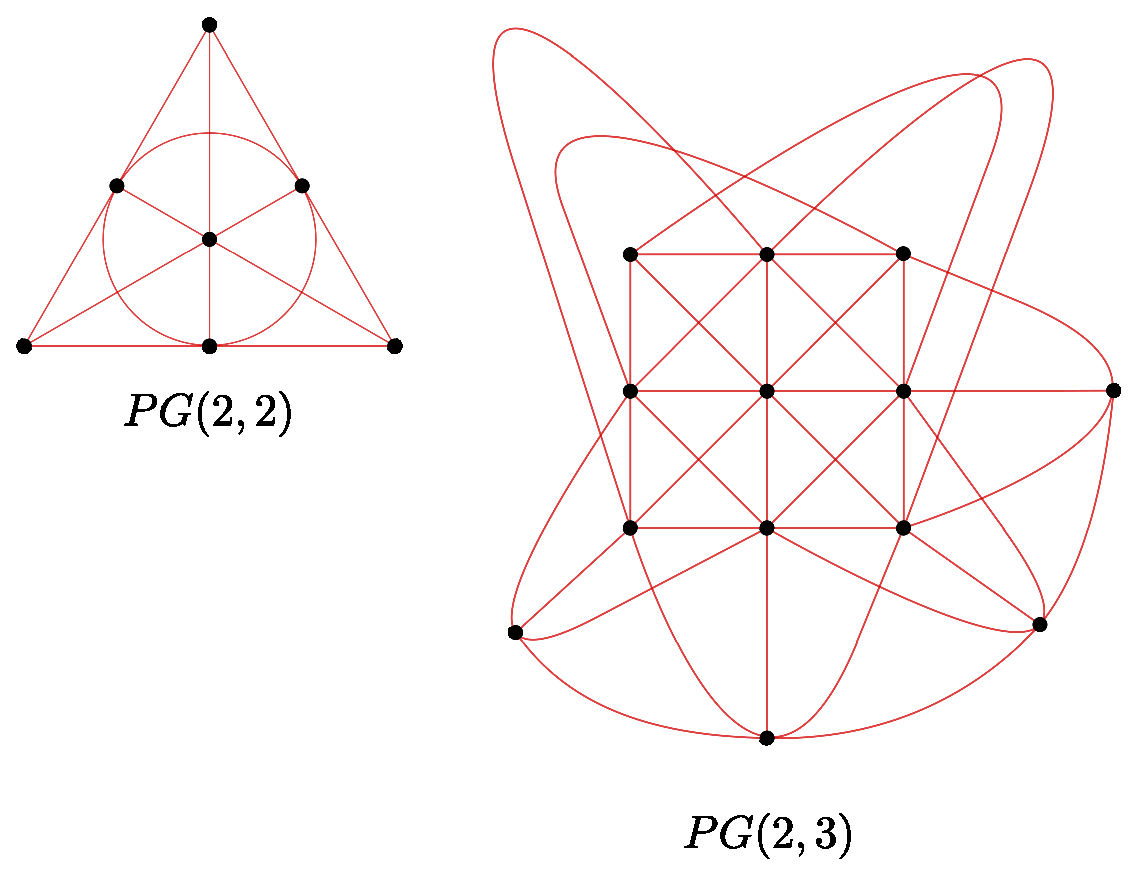
\includegraphics[scale=0.7]{Figures/chapter1/pg(2,2)_pg(2,3).eps}
        \caption{The Fano matroid on the Fano plane together with the matroid on
        $PG(2,3)$.}
        \label{fig_1.14}
    \end{figure}
\end{example}

\begin{theorem}\label{1.5.4}
    Let $M$ be a matroid on a set $E$ having a subset $X$ that is both a circuit
    and ahyperplane. Let $\Bc$ be the collection of bases of $M$, and  $\Bc'=\Bc
    \cup \{X\}$, then $\Bc'$ is the set of bases of a matroid $M'$ on $E$.
    Moreover, if $\Cc$ is the set of circuits of  $M$, then  $M'$ has the
    following as its set of circuits:
    \begin{equation*}
        \Cc'=(\com{\Cc}{X}) \cup \{X \cup e : e \in \com{E}{X}\}
    \end{equation*}
\end{theorem}

There are also necessary and sufficient conditios on which a geometry actually
represents a matroid of rank $\leq 4$.

\begin{theorem}\label{1.5.6}
    A set $E$ together with a collection of lines inducing a geometry on  $E$ is
    a simple matroid of rank at most $4$ if and only if the following hold:
    \begin{enumerate}
        \item[(1)] Any two distinct lines meet in at most one point.

        \item[(2)] Any two distinct planes meeting at more than one point do so
            in a line.

        \item[(3)] Any two distinct lines meeting at a point do so in at most
            one point, and lie on a common plane.

        \item[(4)] Any line not lying on a plane intersects the plane in at most
            one point.
    \end{enumerate}
\end{theorem}

\begin{example}\label{1.20}
    Consider the geometric figures $P$, and $P'$ of figure \ref{fig_1.15}. We
    call the matroid on $P$ a  \textbf{Papus} matroid, while $P'$ is
    non-Papus they both obey law  $1.5.9$, and hence are geometric
    representations of  matroids of $\rank=3$. The Papus matroid $P$ is a
    representable matroid, while the non-Papus matroid  $P'$ is
    nonrepresentable. A ``smallest'' matroid can be derived with this property
    from the affine space $AG(3,2)$.
    \begin{figure}[h]
        \centering
        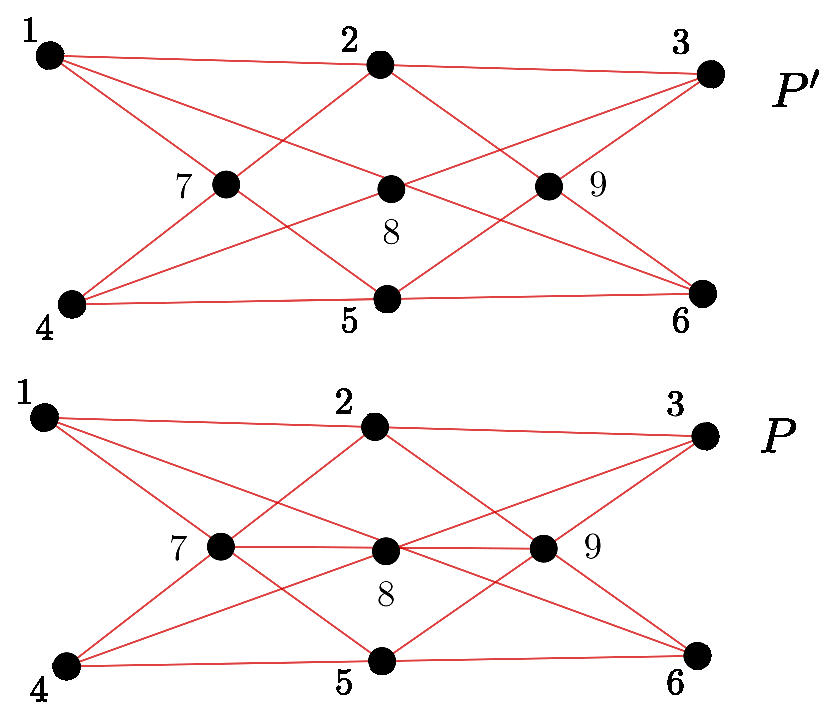
\includegraphics[scale=0.8]{Figures/chapter1/paupus_nonpaupus.eps}
        \caption{$P'$ is a non-Papus matroid, and $P$ is a Papus matroid.}
        \label{fig_1.15}
    \end{figure}
\end{example}

It turns out most of the matroids represented here belong to a specific class of
matroids which we define below.

\begin{theorem}\label{1.5.7}
    Let $E=\{t,x_1,y_1, \dots, x_r,y_r\}$ for some $r \geq 3$. Let
    $\Cc_1=\{\{t,x_i,y_i\} : 1 \leq i \leq r\}$, let
    $\Cc_2=\{\{x_iy_i,x_j,/y_j\} : 1 \leq i \leq j \leq r\}$. Let $\Cc_3$ be the
    possibly empty collection of all $\{z_1, \dots, z_r\}$ such that $z_i \in
    \{x_i,y_i\}$, and no two member of $\Cc_3$ has more than $r-2$ points in
    common. Let  $\Cc_4$ be the collection of all $(r+1)$-element subsets that
    do not contain members of $\Cc_2 \cup \Cc_3$. Then there is a matroid on $E$
    of rank  $r$ having  $\Cc=\Cc_1 \cup \Cc_2 \cup \Cc_3 \cup \Cc_4$ as its
    collection of circuits.
\end{theorem}
\begin{proof}
    We have that $\emptyset \notin \Cc$, as the only collection that can
    possibly be empty is  $\Cc_3$. We also have by definition that no member of
    $\Cc$ can be a proper subset of another member of  $\Cc$.

    Now if  $\Cc$ were the collection of circuits on  $M$, then we have that
    $\rank{M} \leq r$,by definition of $\Cc_4$. On the otherhand, by the
    definition of $\Cc_3$, at most one of the subsets $\{y_1, \dots, y_r\}$ and
    $\{y_1, \dots, y_{r-1}, x_r\}$ is independent, so that $\ranbk{M} \geq r$.
    This makes $\rank{M}=r$.

    Now, let $C_1, C_2 \in \Cc$, and $e \in C_1 \cap C_2$. If $C_1,C_2 \in \Cc_1
    \cup \Cc_2$, then the weak circuit elimination axiom is satisfied. Now,
    suppose then that $|C_1| \leq |C_2|$ and that $C_2 \in \Cc_3 \cup \Cc_4$.
    Then we have:
    \begin{align*}
        |\com{(C_1 \cup C_2)}{e}|  &=   |C_1 \cup C_2|-1 \\
                                &= |C_1|+|C_2|-|C_1 \cap C_2|-1 \\
                                &= |\com{C_1}{C_2}|+|C_2|-1
    \end{align*}
Since $|C_2|=r$ or $|C_2|=r+1$, we must have that  $|\com{(C_1 \cup C_2)}{e}|
\geq r+1$, or that $C_2 \in \Cc_3$ and that $|\com{C_1}{C_2}|=1$. In the first
case, we get that there is a circuit $C \in \Cc$ contained in
$\com{(C_1 \cup C_2)}{e}$. In the second case, we get that $C_2 \in \Cc_4$,
making $|C_1|>|C_2|$, which contradicts our suposition, so only the first case
is true. This makes the collection $\Cc$ into the collection of cirvuits of
$M$.
\end{proof}

\begin{definition}
    A matroid $M$ on a set $E$ having as collection of circuits the collection
    $\Cc$ defined in theorem \ref{1.5.7} an  \textbf{$r$-spiked matroid} with
    \textbf{tip} $t$, and legs  $L_i=\{t,x_i,y_i\}$ where $1 \leq i \leq r$. If
     $\Cc_3=\emptyset$, then we call $M$ a  \textbf{free spike}. If
     $/M'=\com{M}{t}$ is also a matroid, then we call $M'$ a \textbf{tipless}
     spiked matroid.
\end{definition}

\begin{theorem}\label{1.5.8}
    Let $r \geq 2$ be an integer. A matroid  $M$ is an  $r$- spike with tip $t$
    if, and only if:
    \begin{enumerate}
        \item[(1)] $E$ is the union of the legs  $L_1, \dots, L_r$, each of
            which is a $3$-element circuit containing  $t$.

        \item[(2)] For each $1 \leq k \leq r-1$, the union of any  $k$ legs
            $L_1, \dots, L_r$ has rank $k+1$.

        \item[(3)] $\rank{(L_1 \cup \dots \cup L_r)}=r$.
    \end{enumerate}
\end{theorem}

\begin{definition}
    Let $M$ be a matroid. We call distinct elements  $e$ and  $f$ of  $M$
    \textbf{clones} if there exists an isomorphism $\phi:M \rightarrow M$ of $M$
    onto itself such that $\phi:e \rightarrow f,f \rightarrow e$, and $\phi:g
    \rightarrow g$ for any $g$ distinct from both  $e$ and  $f$.
\end{definition}
